% ------------ HEADER ------------ %


% PROJECT: Today I Learned Document
% AUTHOR: Miles Smith


% ------------ PREAMBLE  ------------ %


\documentclass[12pt]{report}
\usepackage{times}
\usepackage[margin=1.5in]{geometry}
\usepackage{amsmath,amsthm,amssymb}
\usepackage[version=4]{mhchem}
\usepackage{graphicx}
\usepackage{multirow}
\usepackage{setspace}
\usepackage{subcaption}
\usepackage{caption}
\usepackage{float}
\onehalfspacing


% ------------ DOCUMENT ------------ %

\begin{document}

\begin{center}
\huge{\textbf{Today I Learned}}\\
\large{An insight into the fun things I am learning and doing}\\

\vspace*{0.5cm}
\textbf{Miles Smith}\\

\vspace*{1cm}
\textbf{Introduction}\\
\textit{In an attempt to better document the things that I am learning and help things stick with me, I am hoping to create this running document so I can ramble about whatever cool things I learn each day.}\\
\vspace*{2cm}
\clearpage

\tableofcontents

\clearpage

\end{center}

\chapter{Being a Masters Student at Stanford \\ in Civil and Environmental Engineering}

\clearpage

\section{Monday, March 7, 2022}
\par
An interesting topic that I was reading about today is “ionocraft” which are airplanes propelled by ion propulsion systems that have no moving parts. This article by Steven Barrett’s group shows a proof of concept on how a heavier than air craft can be propelled by ionic wind. From my understanding, it works by using high-voltage electrodes (20 kV+?) to ionize air (mostly N2) and accelerate the ions across the electric field to the negative electrode.  The thrust force is generated as a reaction to the motion of the ions. In their proof-of-concept tests, the craft traveled between 40-45 meters in 8-9s before turning the thruster off.

\begin{figure}[H]
\centering
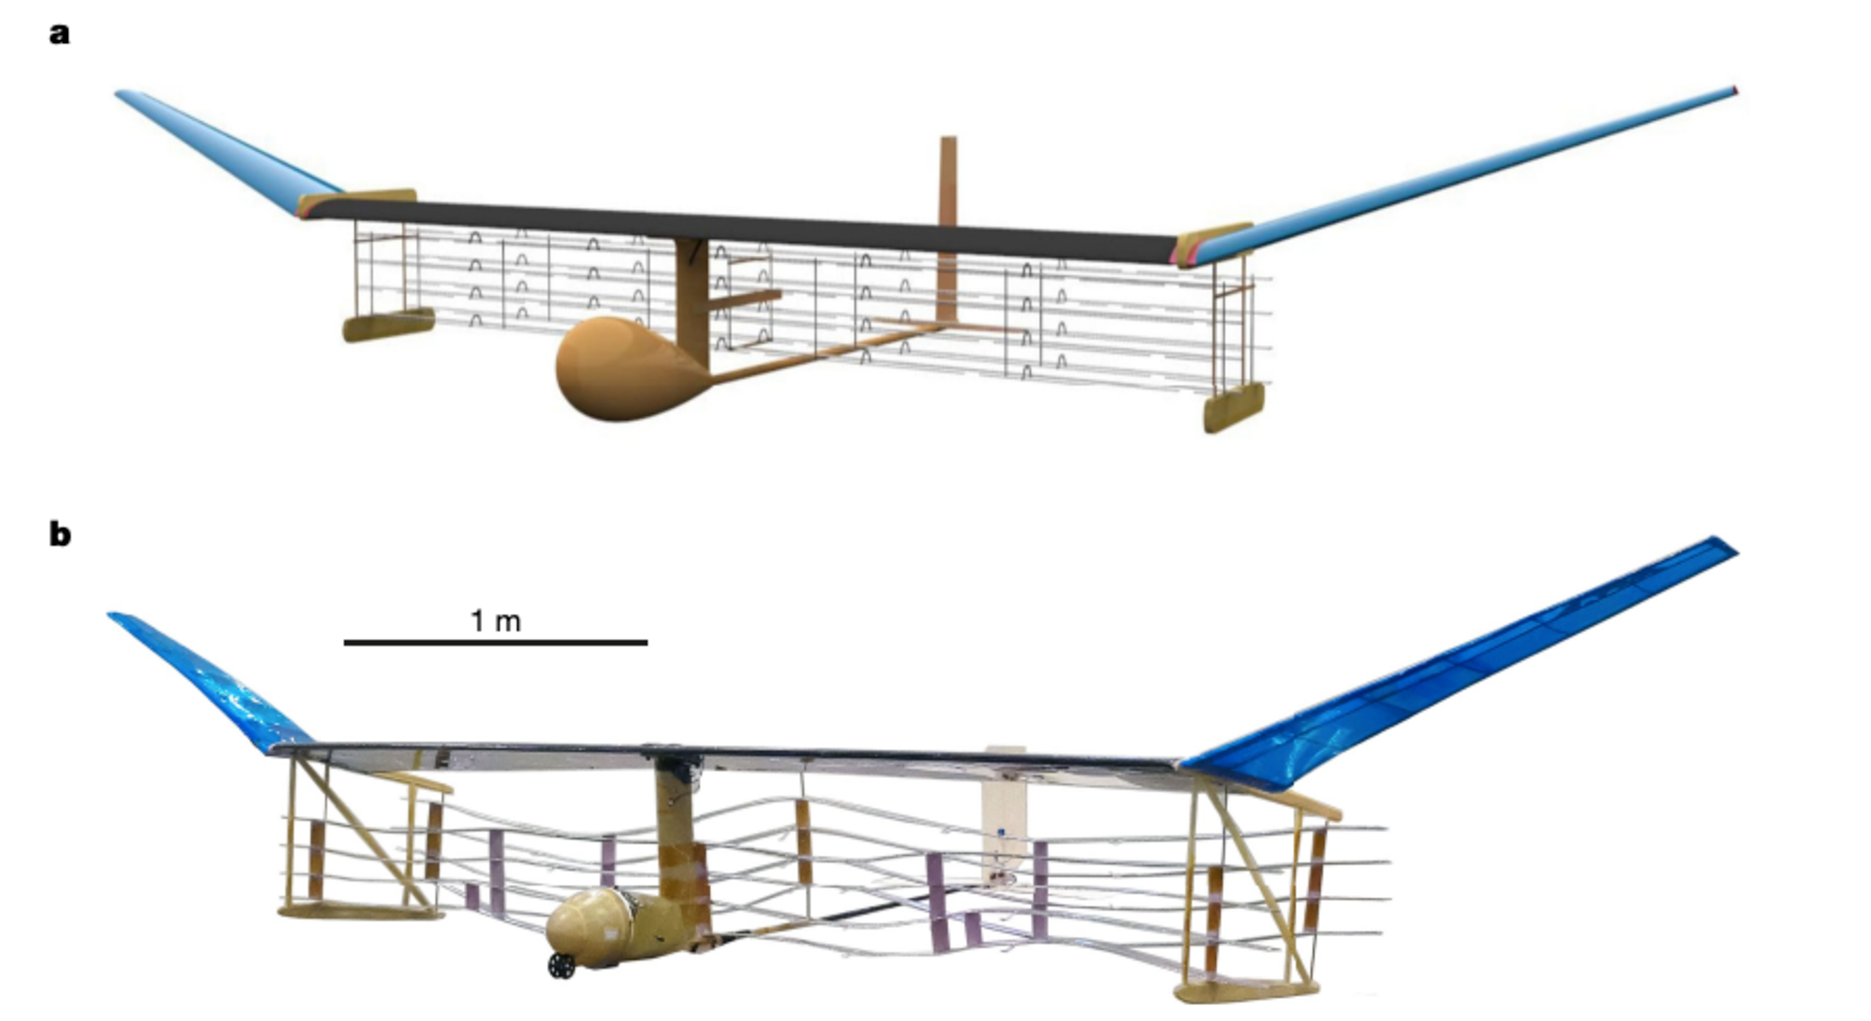
\includegraphics[width=\linewidth]{images/ionicwindplane.pdf}
\end{figure}

\begin{figure}[H]
\centering
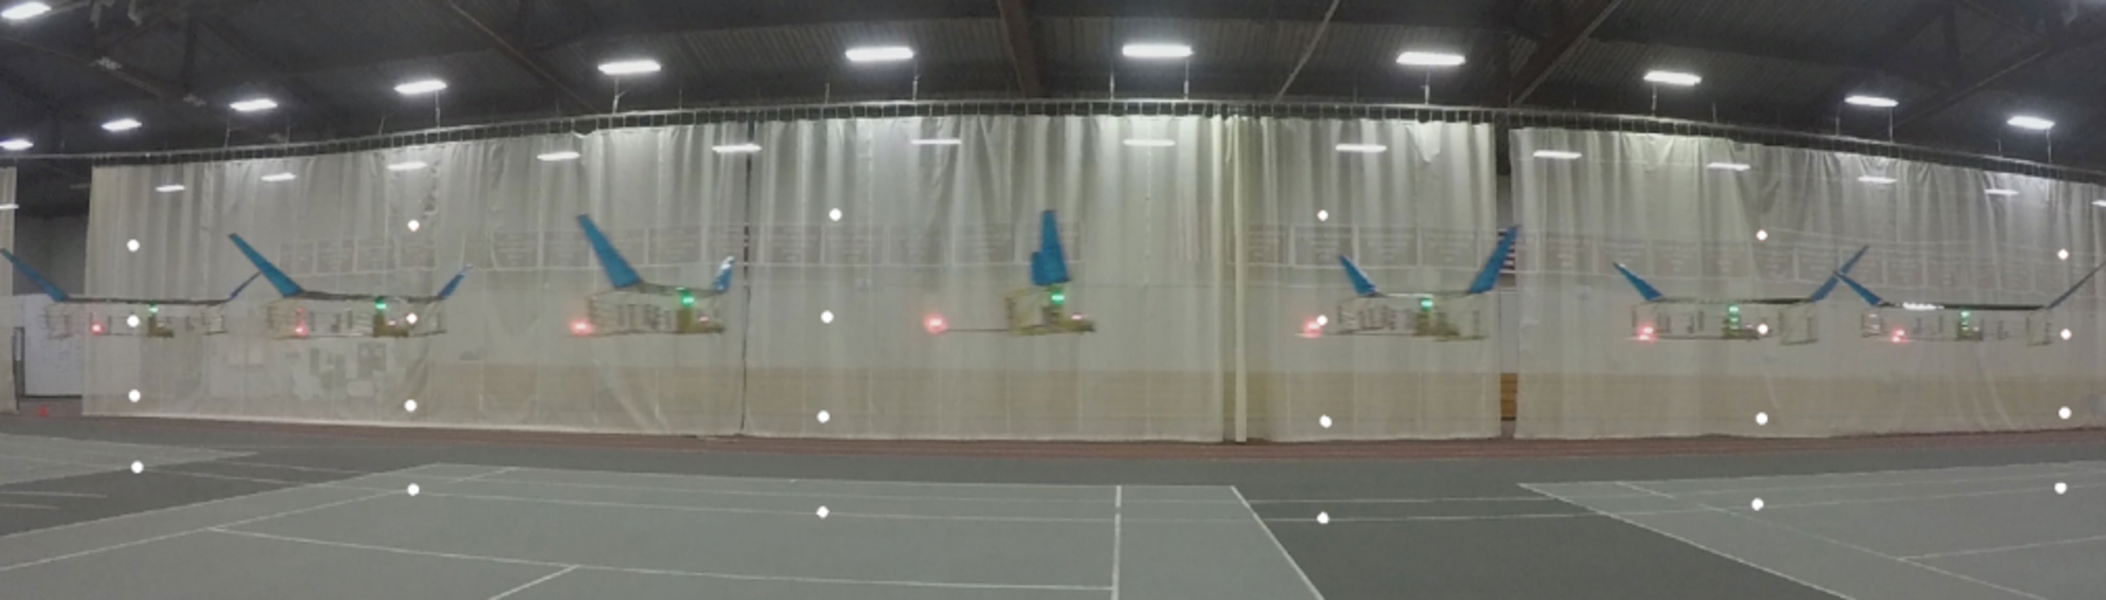
\includegraphics[width=\linewidth]{images/ionocraftmotion.pdf}
\end{figure}

\par
Today I also spent some time working on a computational fluid mechanics problem set for my Physics of Wind course. Given collected over a domain and assuming horizontally homogeneity I spatially averaged the data to study potential temperature and vertical velocity as a function of altitude in the atmospheric boundary layer. One part of the assignment involves applying similarity relationships to estimate the convective velocity scale and the surface heat flux, but I am not exactly sure how to do that. 

\section{Tuesday, March 8, 2022}
\par
To continue on yesterday’s discussion about solid-state propulsion, Barrett’s group used a corona discharge thruster to propel the aircraft. This works by applying a DC voltage across two asymmetric electrodes as shown, where the positive electrode is a wire that ionizes air molecules within some radius, referred to as the corona (is this related to the Debye length?) and the negative electrode is some sort of mesh material. Ionized materials then move along the induced electric field and collide with neutral air molecules to produce in the opposite direction of ion flow. 

\begin{figure}[H]
\centering
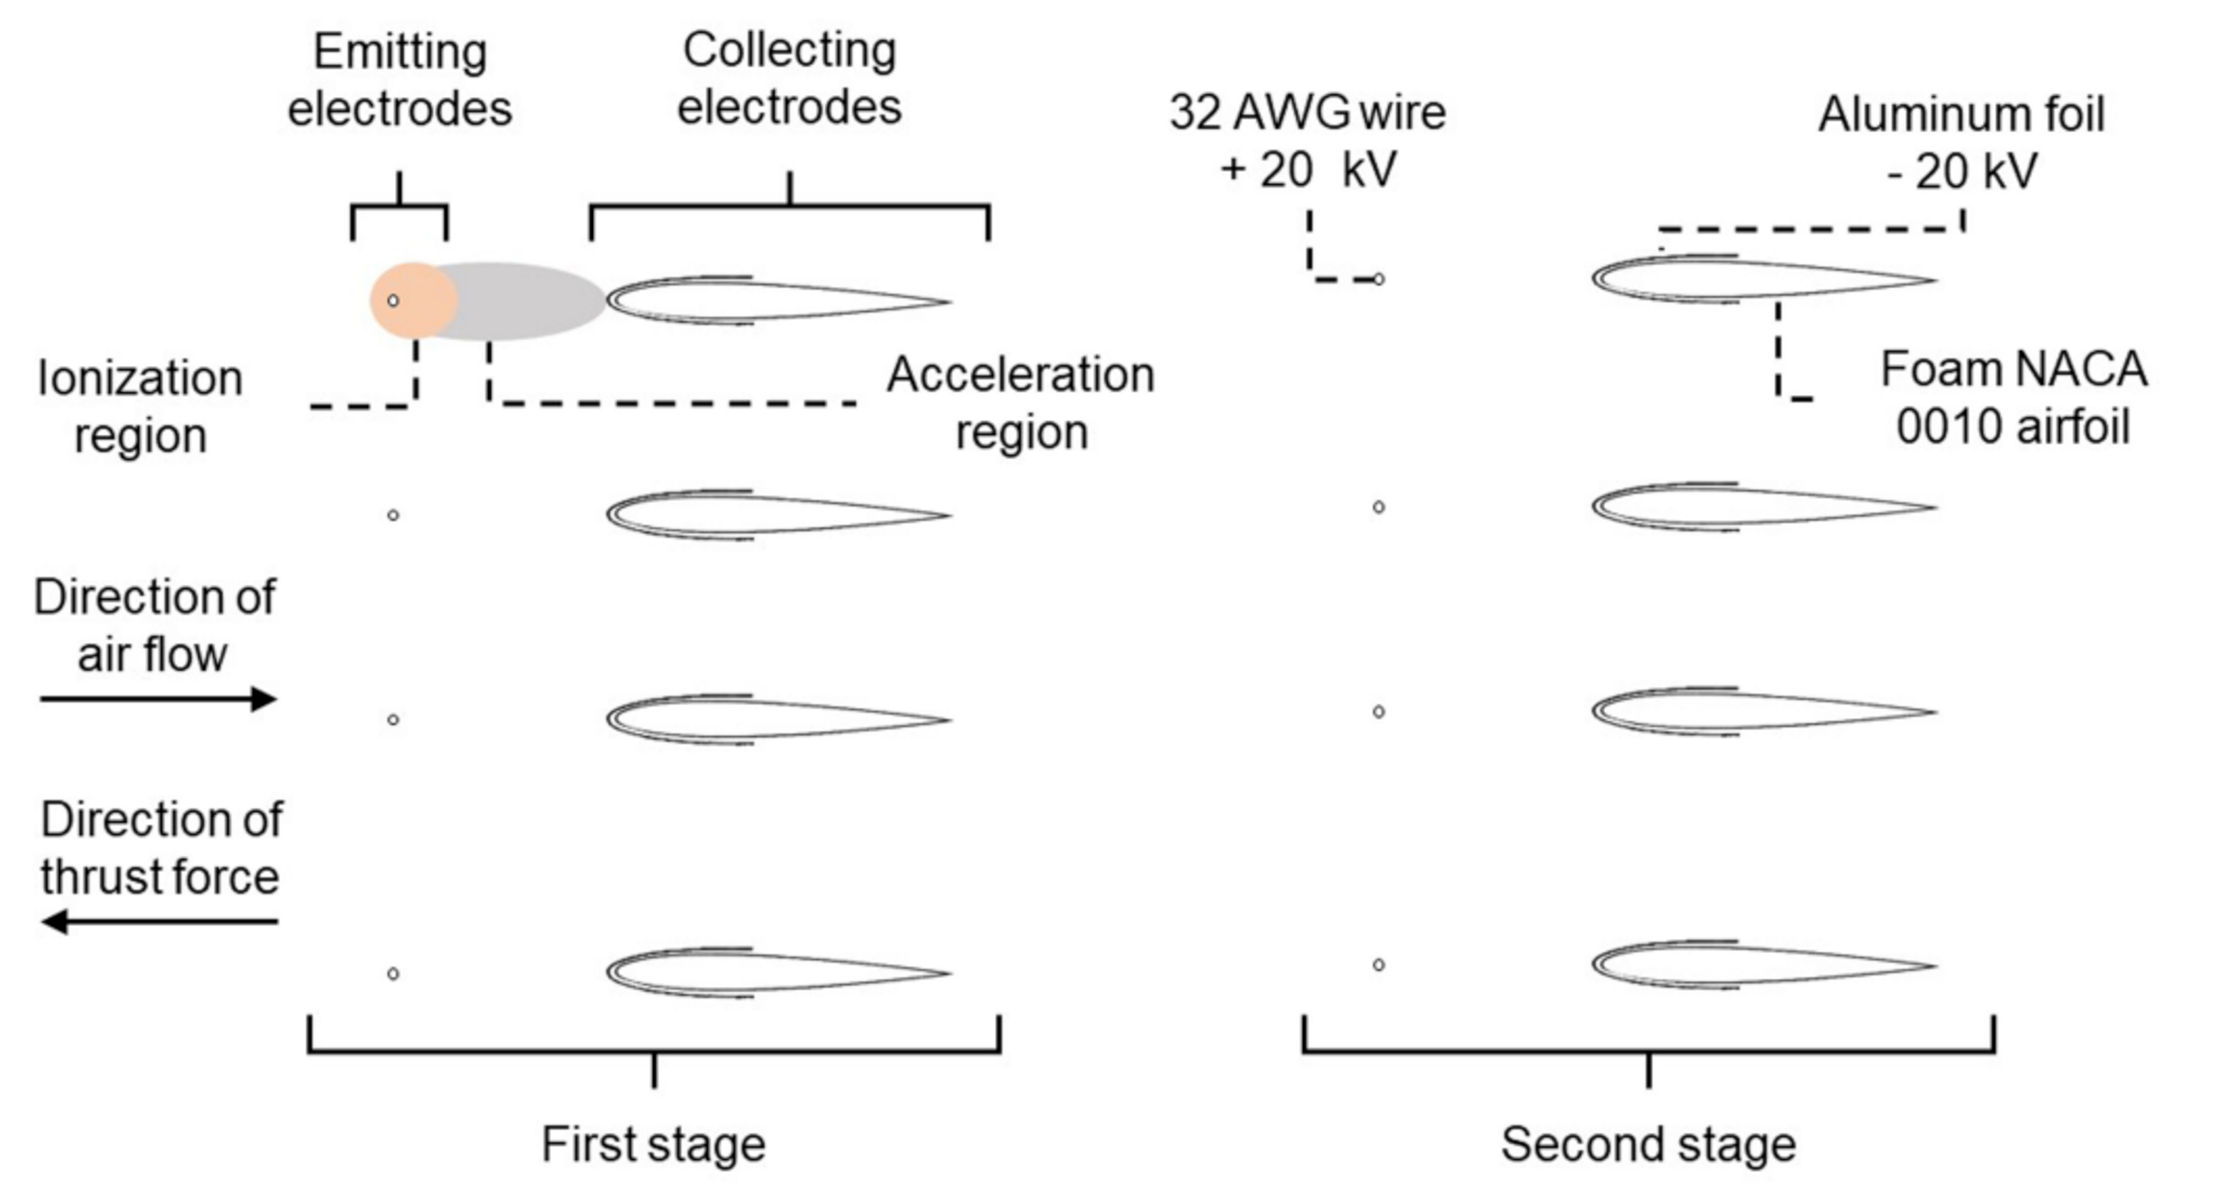
\includegraphics[width=\linewidth]{images/thrustdiagram.pdf}
\end{figure}

\par
However, in their paper, \textit{A dielectric barrier discharge ion source increases thrust and efficiency of electroaerodynamic propulsion}, they note that a corona discharge can be limited by two processes (1) a minimum electric field at the emitter for ionization and (2) a maximum space charge density arising from the self-limiting nature of electric-field driven charge flow. Thus, they proposed a decoupled system using a dielectric barrier discharge plasma where ions are produced by a separate ``emitter." By using a decoupled thrusted more current can be produced and, as a result, more thrust. 

\begin{figure}[H]
\centering
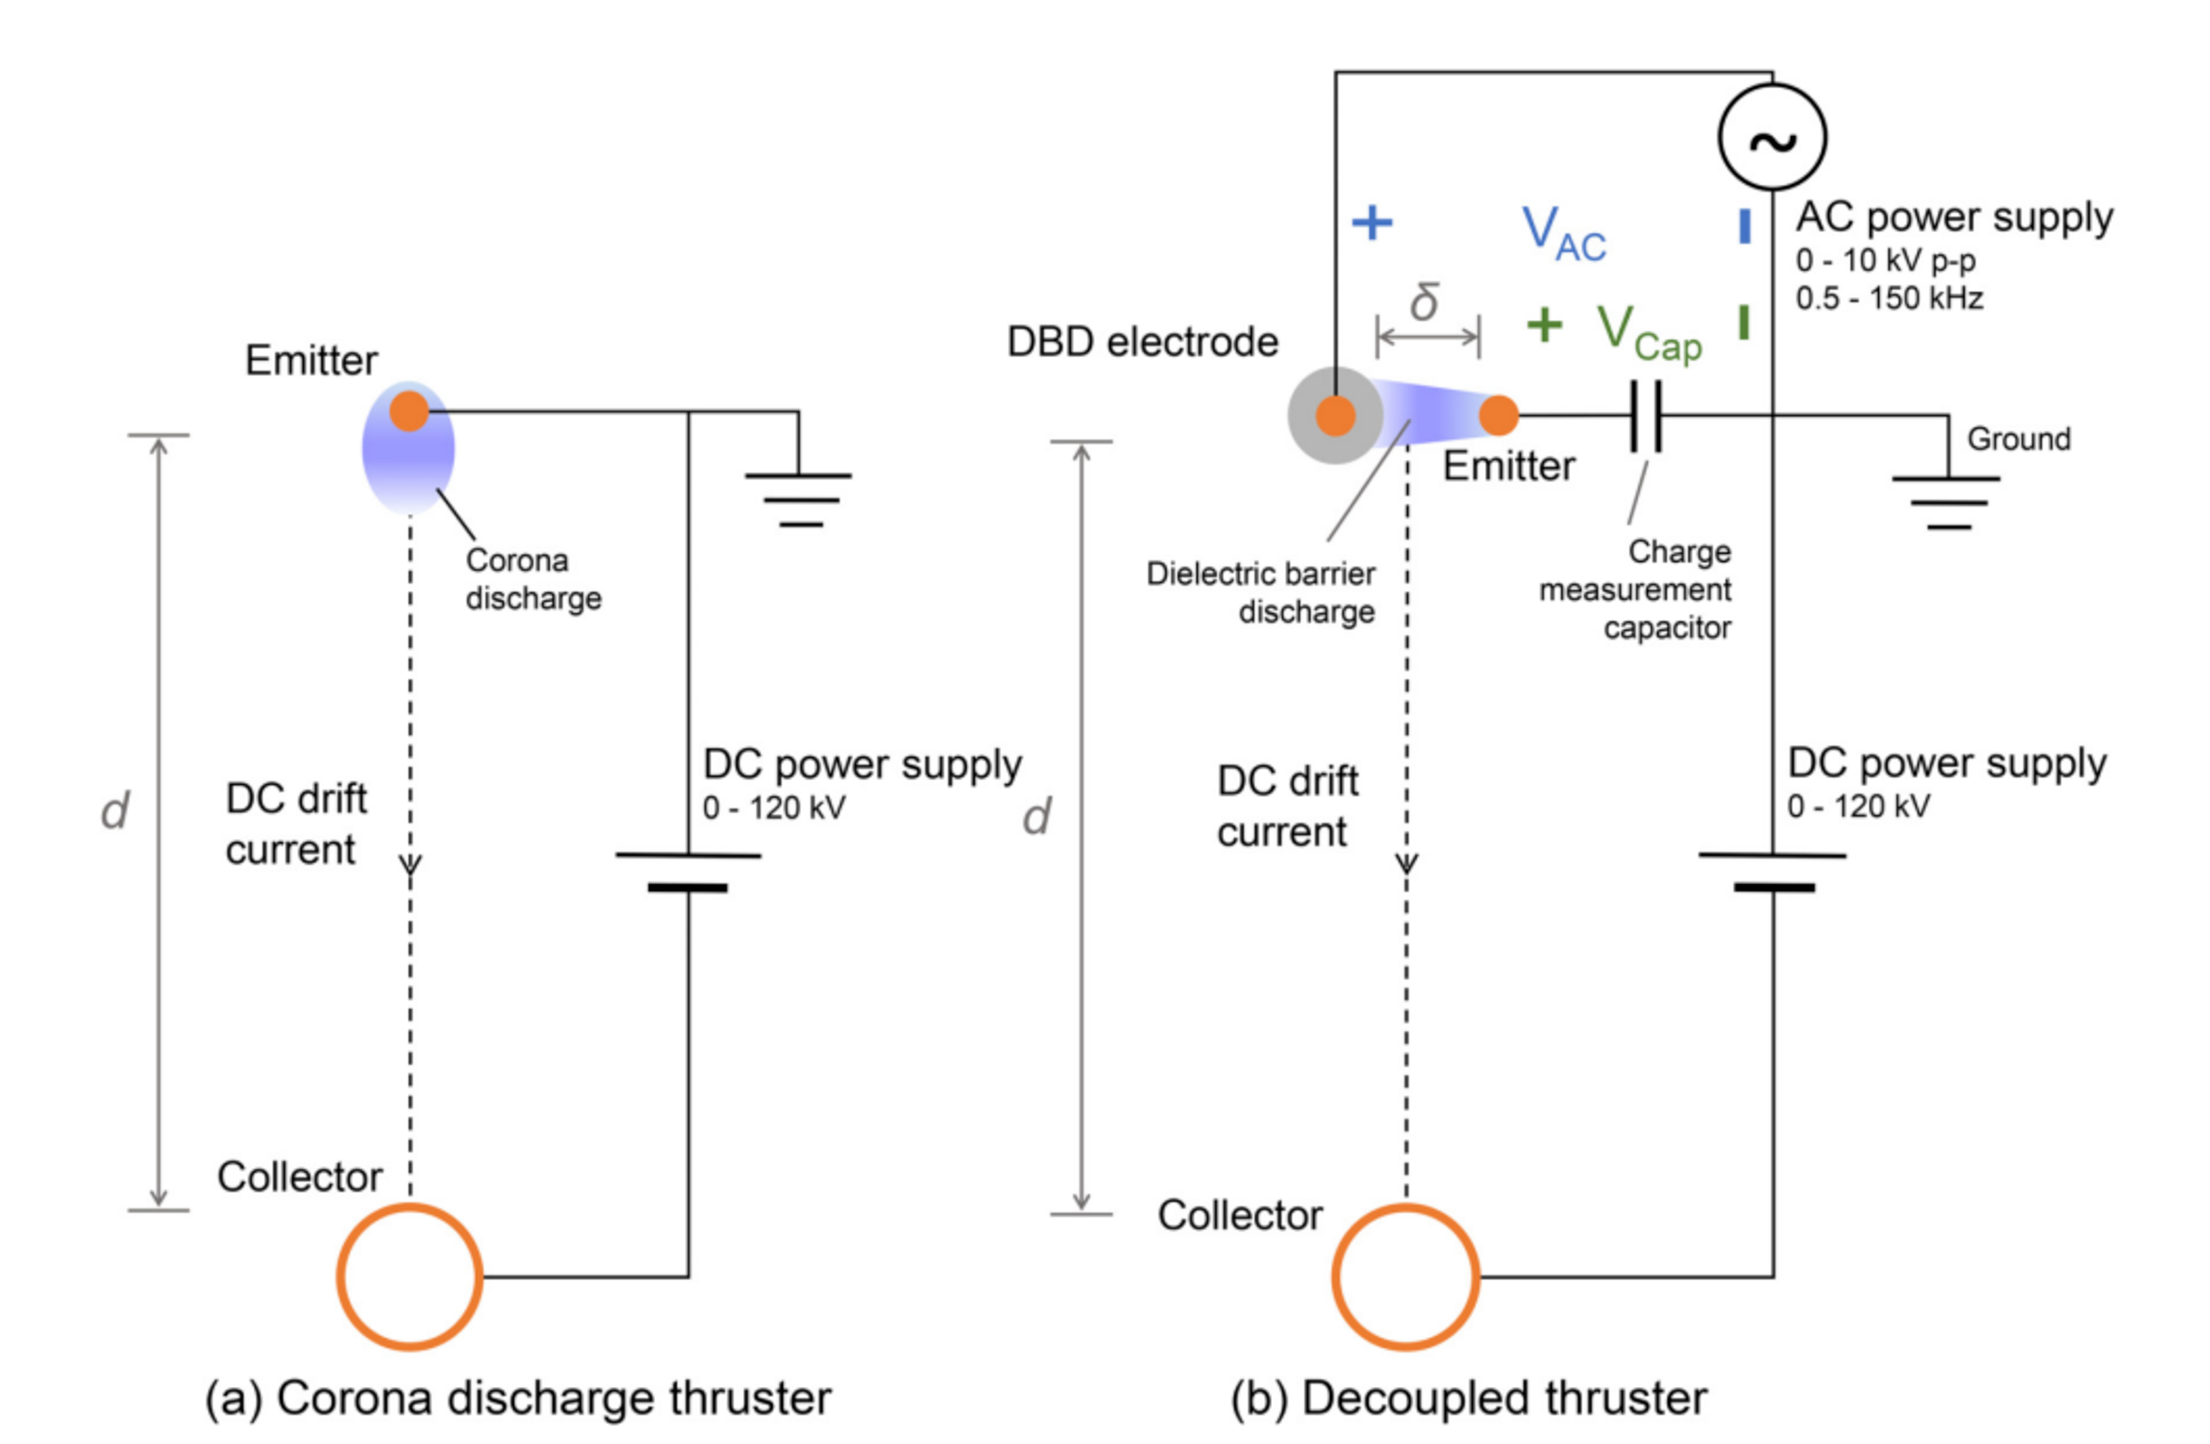
\includegraphics[width=\linewidth]{images/dbd thruster schematic.pdf}
\end{figure}

\section{Wednesday, March 9, 2022}

\par
An interesting article on Nature titled \textit{Flying with ionic wind} discussed how the ionocraft at MIT was developed. One of the big challenges with the ionocraft seems to be optimizing the weight so that the thrust from the corona is strong enough to create some lift.  This is probably why the scalability of the ionocraft is uncertain.  The original design was generated through some geometric parameter optimization algorithm to determine the optimal wing span and mass for the thrust generated.  One of the big challenges seems to be that takeoff is very hard and inefficient but once in flight the efficiency of ionic wind significantly increases making it more feasible. In their experiments, they reported an energy efficiency of only ~2\%, but it is believed that at high speeds the energy efficiency can be as high as 50\%. An interesting thing to note is that it can also be coupled with battery technologies to use electricity from batteries to possibly launch the plane and then use ionic wind propulsion as a secondary energy source.

\begin{figure}[H]
\centering
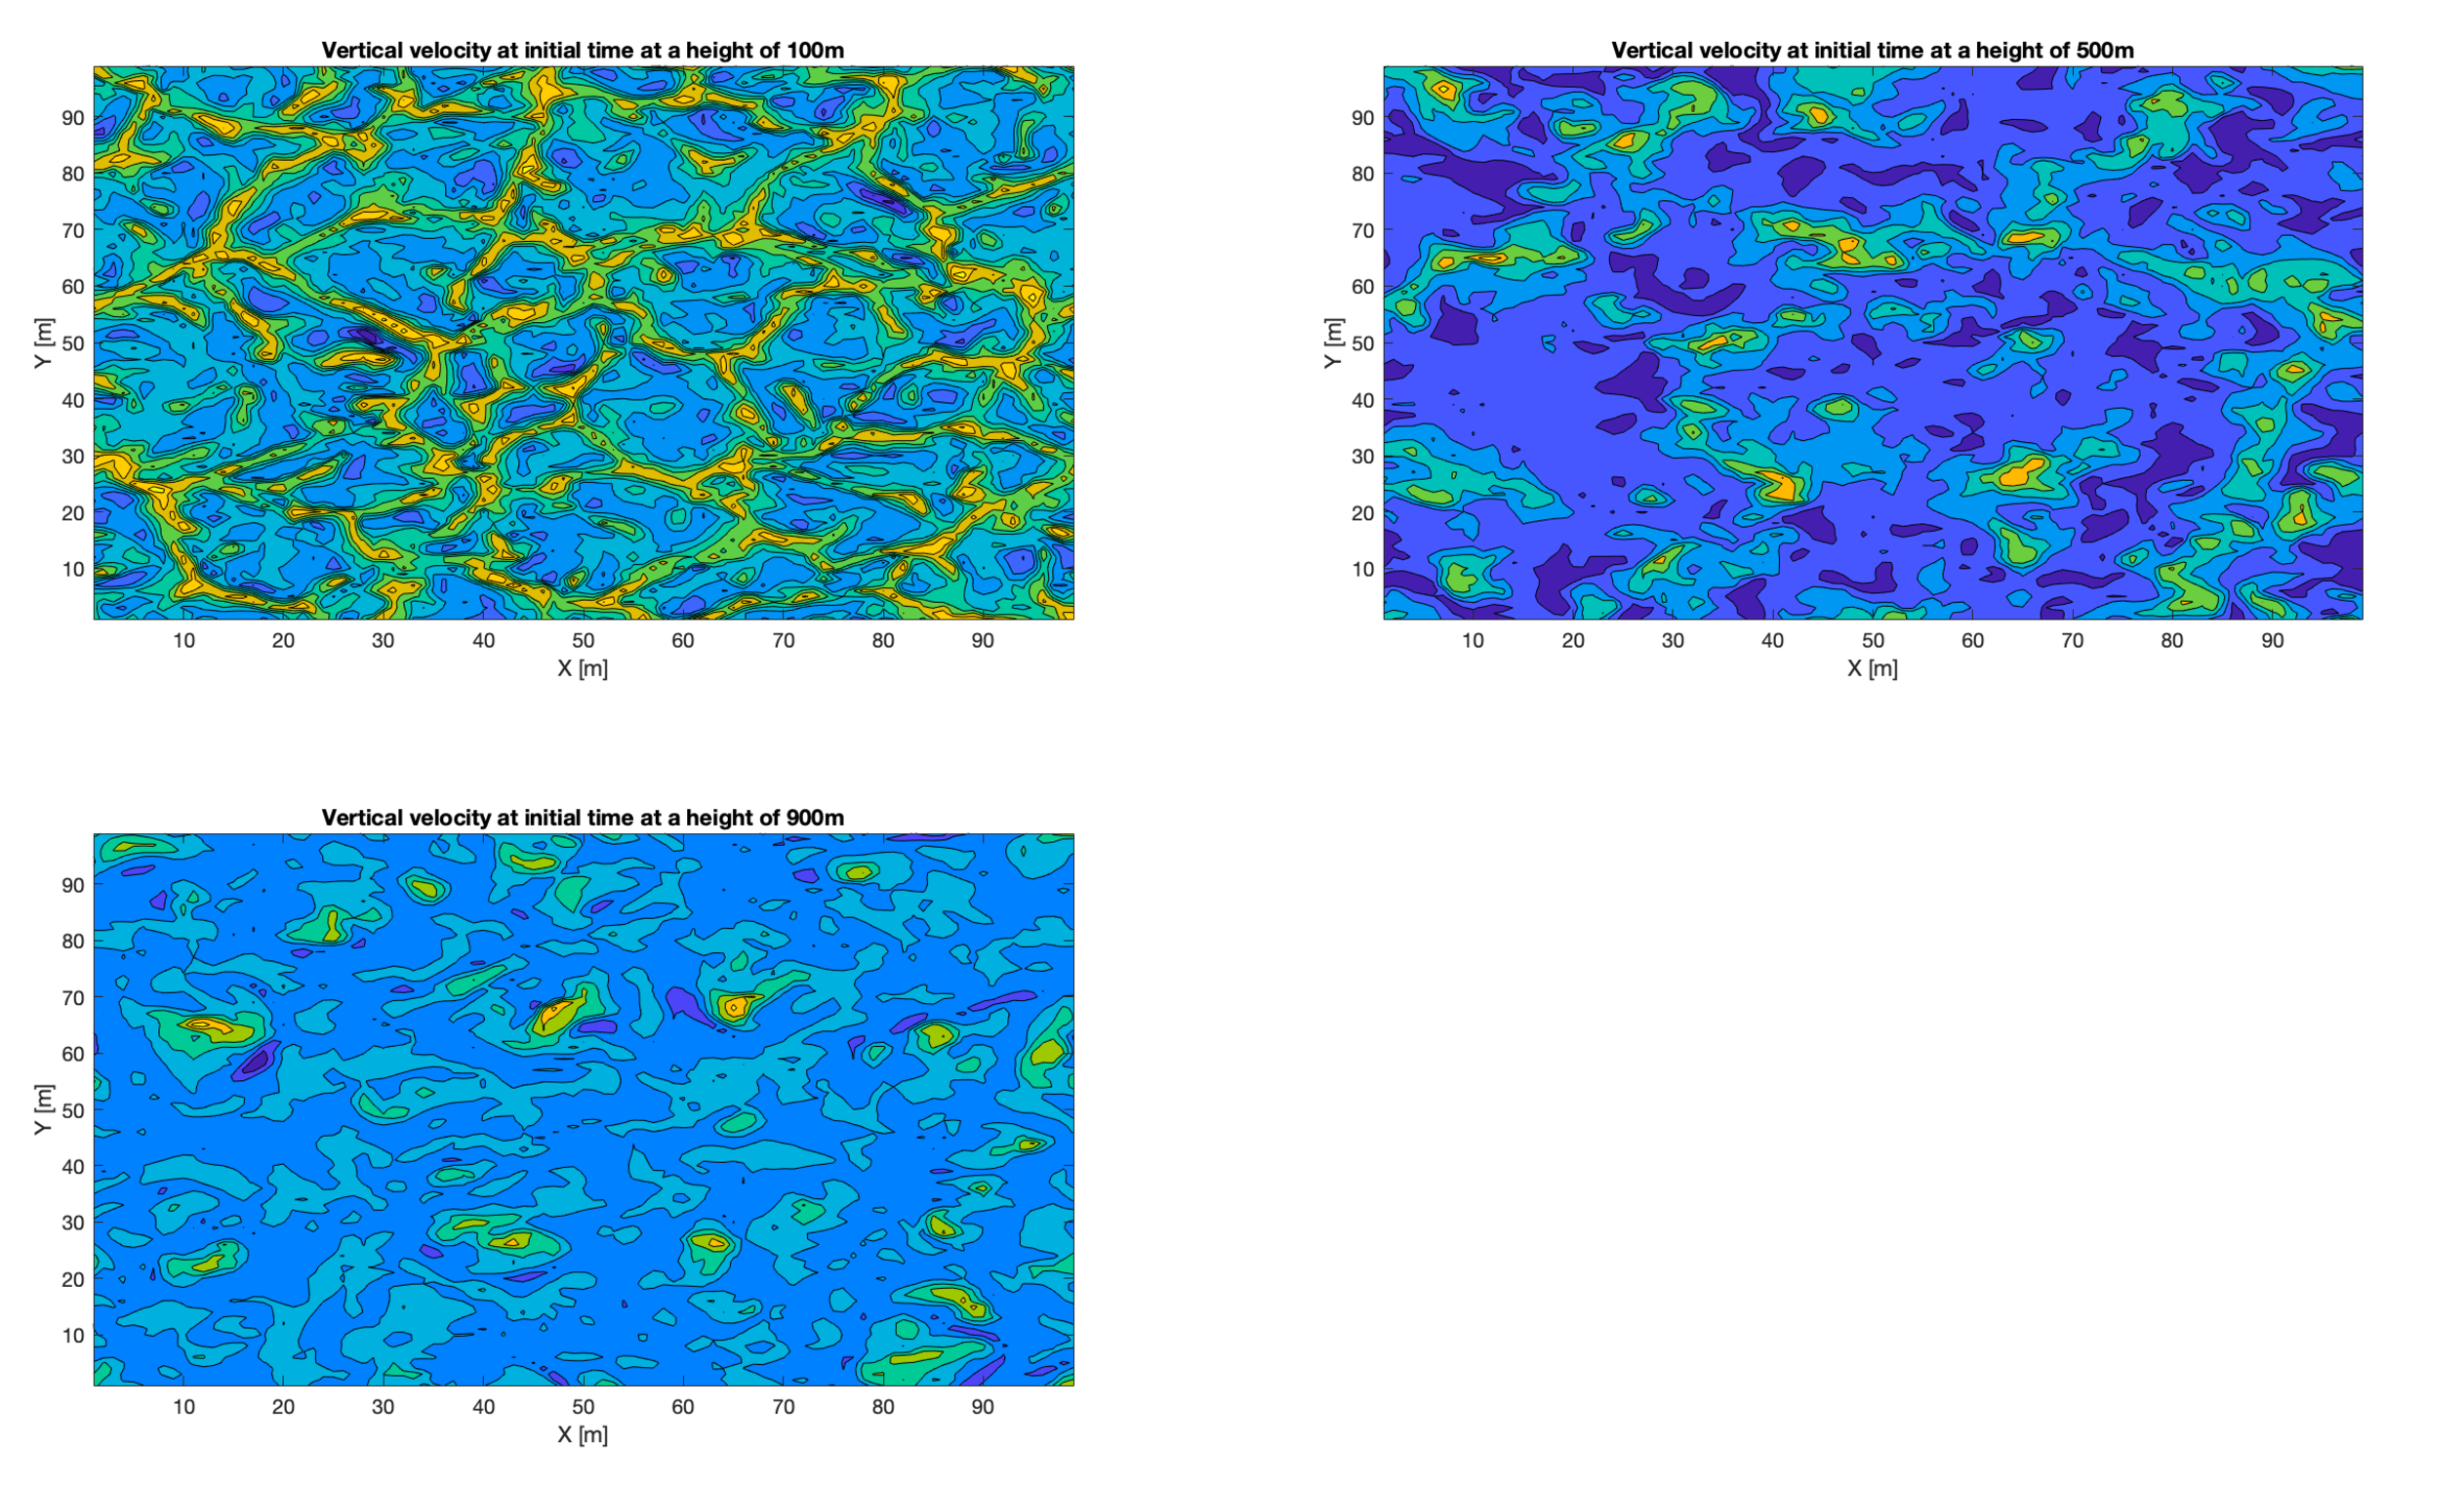
\includegraphics[width=\linewidth]{images/vertical_velocity_contour.pdf}
\end{figure}

\par
In Physics of Wind I am still looking at the large eddy simulations of a "quasi-steady free-convection ABL" that we can allegedly assume is horizontally homogeneous and does not evolve much temporally. Here are some interesting figures of how the vertical velocity profile changes (at the initial time) with height in the ABL.

\begin{figure}[H]
\centering
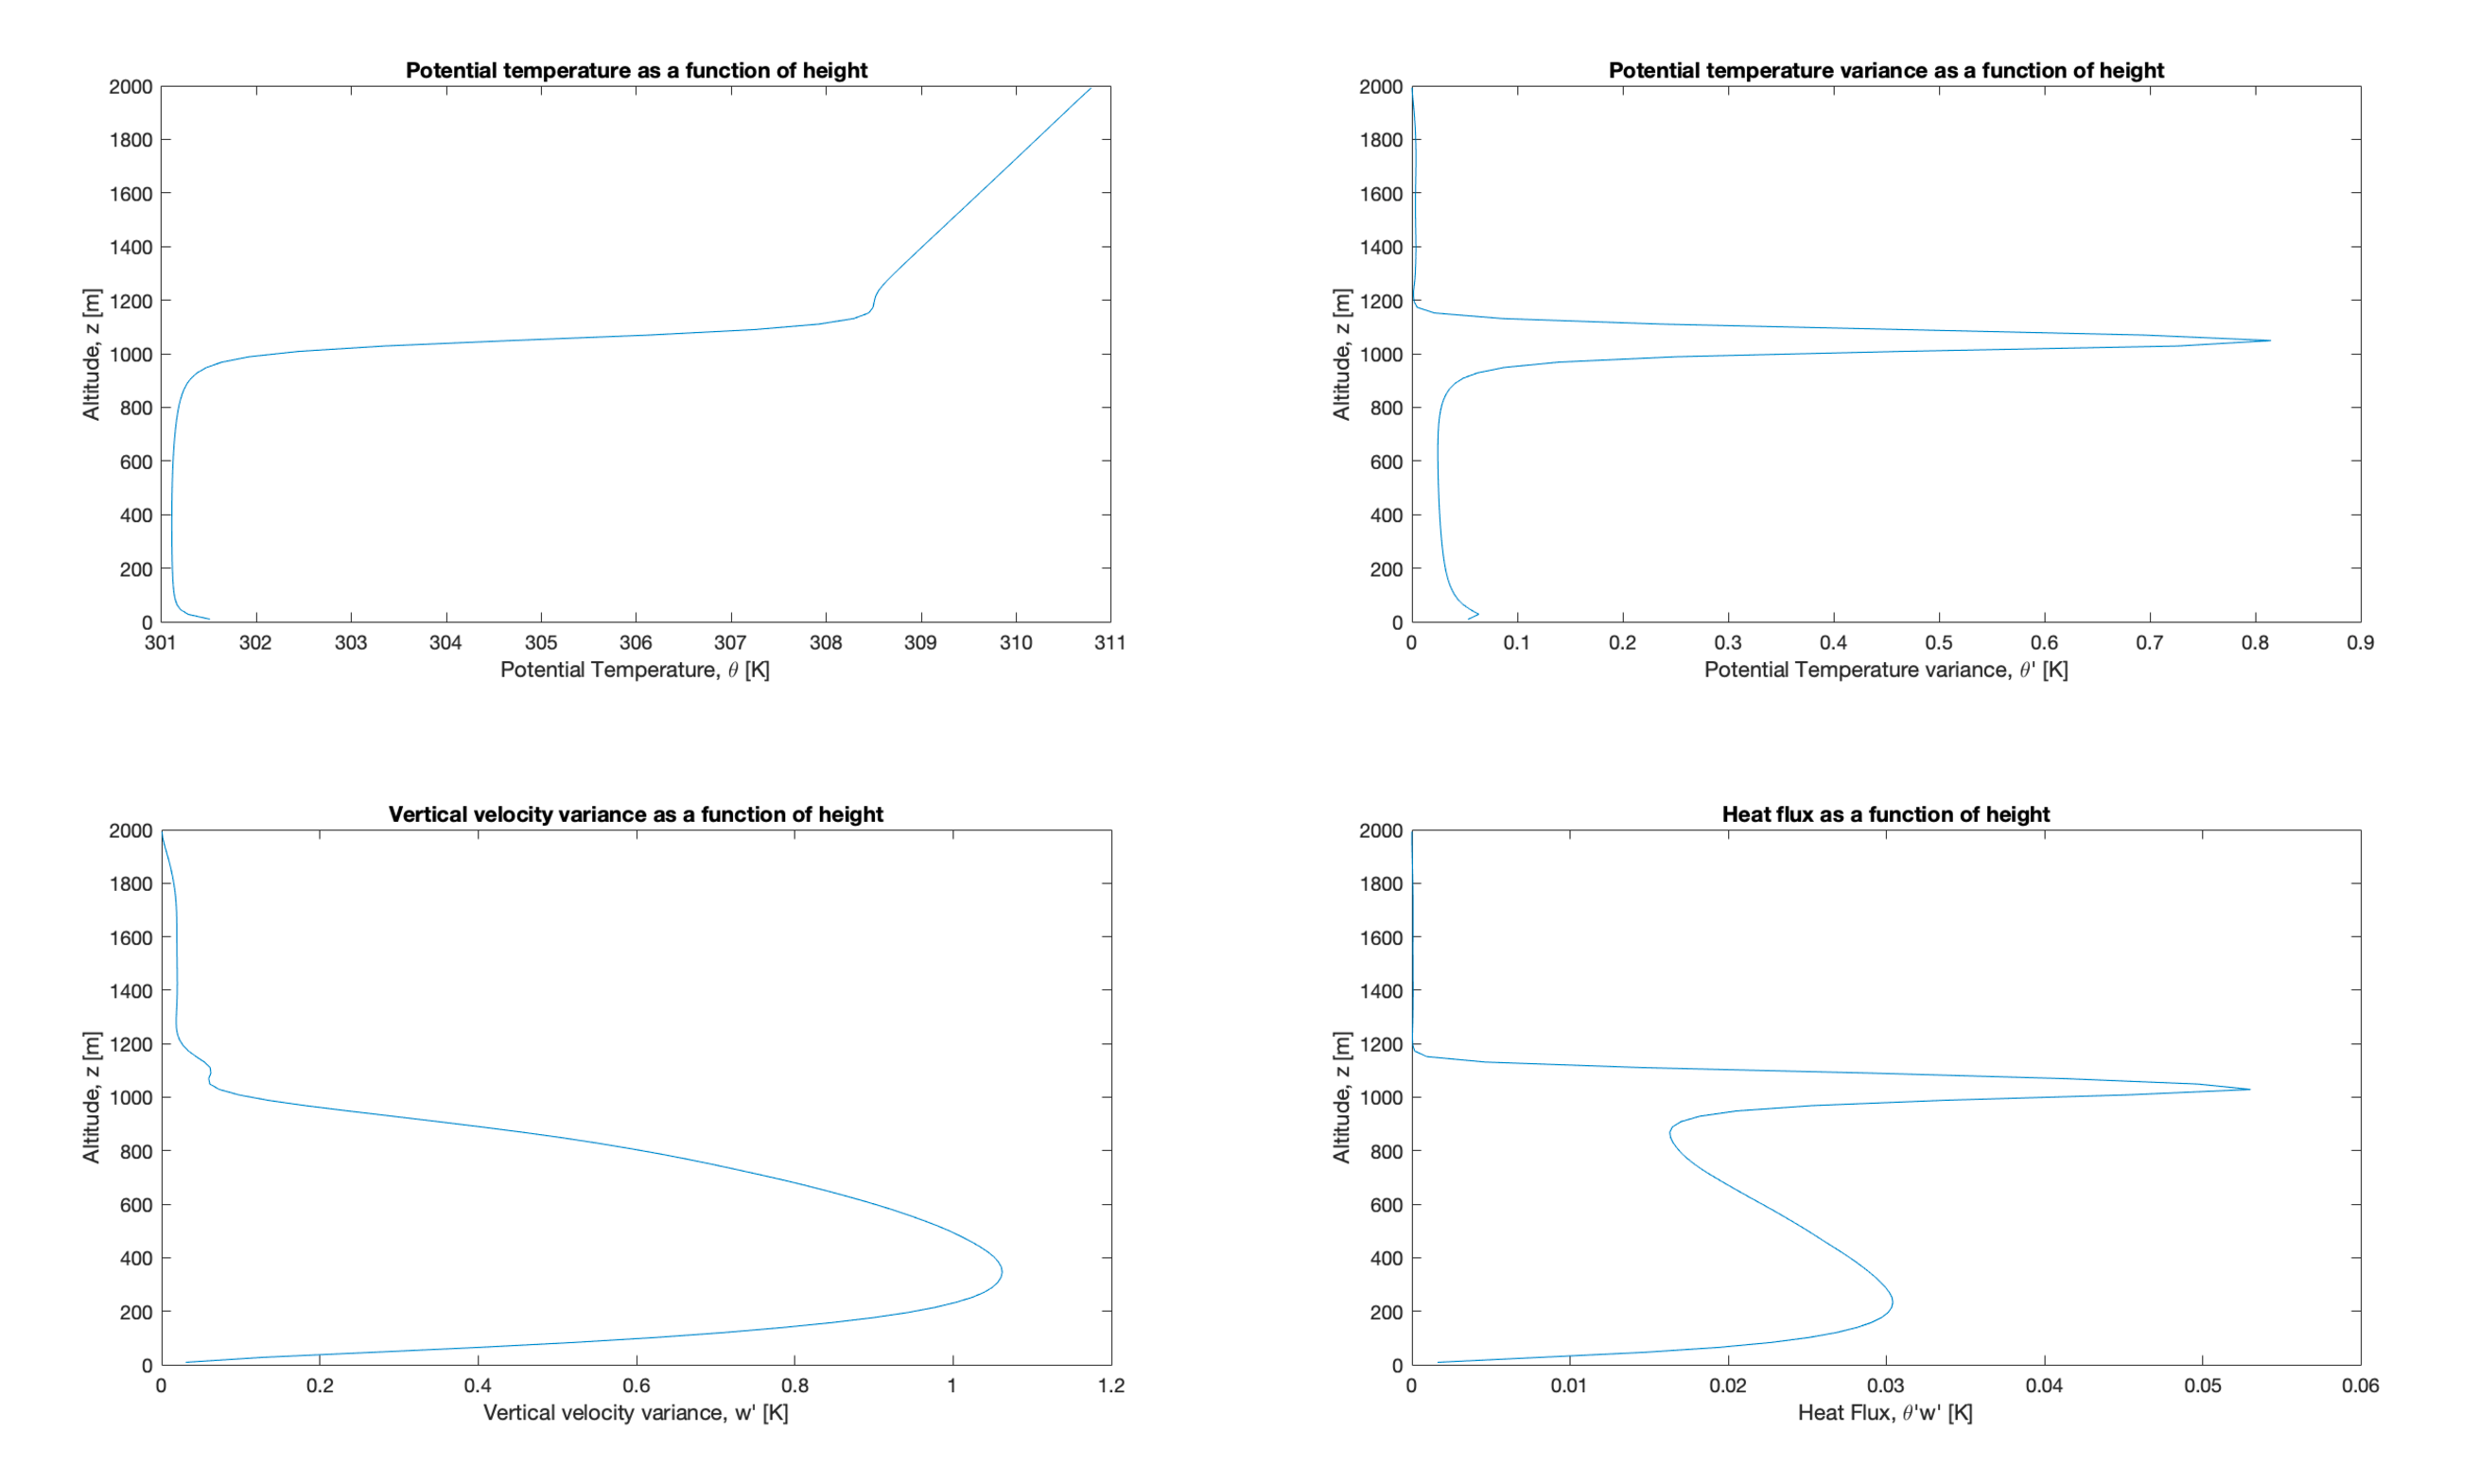
\includegraphics[width=\linewidth]{images/ABL_Vertical_Profiles.pdf}
\end{figure}


\section{Thursday, March 10, 2022}

\par
Today was the last day of classes for the winter quarter, which is an exciting and unsettling feeling. Will I be able to stay at Stanford and do a Ph.D. here? Will I go to MIT? Will I ever be able to schedule a meeting with Mark, Ted, and Erik? There is a bit of time to deal with this but really not a whole lot since I need to put together an application relatively soon. Nothing I can do about it tonight, but maybe I should bump Ted in the morning tomorrow. Anyway, today I learned a bit too much about Euler's identity, Euler's equations and trig properties to solve a single plasma physics problem.  As a note, Euler's identity says:

\begin{equation}
\centering
e^{i\pi} = -1, 
\end{equation}

and Euler's equation states that:

\begin{equation}
\centering
e^{i\theta} = \cos(\theta) + i \sin(\theta).
\end{equation}

By adding 

\begin{equation}
\centering
e^{i\theta} = \cos(\theta) + i \sin(\theta)
\end{equation} 

to 

\begin{equation}
\centering
e^{-i\theta} = \cos(-\theta) + i \sin(-\theta) = \cos{\theta} - i\sin(\theta)
\end{equation}

Euler's less intuitive relationships can also be derived which state that:

\begin{equation}
\centering
\cos(\theta) = Re(e^{i\theta}) = \frac{e^{i\theta}+e^{-i\theta}}{2}
\end{equation}

and

\begin{equation}
\centering
\sin(\theta) = Im(e^{i\theta}) = \frac{e^{i\theta} - e^{-i\theta}}{2i}
\end{equation}

The plasma wave table handout is also a blessing to help explain which types of waves will propagate in a plasma under a given set of conditions. I have much to learn about plasma waves I think. 

\section{Friday, March 11, 2022}

\par
What is the difference between Gauss's Law and Poisson's Equation for electrostatics? The big difference is that (in the differential form) Gauss's Law:

\begin{equation}
\centering
\nabla \cdot E = \frac{\rho}{\epsilon_0}
\end{equation}

is a general expression that should always be true. In contrast, Poisson's Equation assumes that there is no magnetic field (thus, it is electrostatic). This assumption states that 

\begin{equation}
\centering
\nabla \times E = 0,
\end{equation}

and subsequently,

\begin{equation}
\centering
E = - \nabla \phi,
\end{equation}

which can be substituted into Gauss's Law to give,

\begin{equation}
\centering
\nabla^2\phi = -\frac{\rho}{\epsilon}.
\end{equation}

Since it is based on an electrostatic assumption, Poisson's equation for electrostatics is not always true. 

\par
Anyway, to continue this seemingly lengthy discussion on ionic wind propulsion, one research group cited using a dielectric barrier discharge plasma, instead of a corona discharge plasma to reduce the applied voltage requirement. However, it seems like the DBD plasma might be less effective for high-speed airflow control, which is important for full-scale airplanes.  It might be useful for smaller, slower UAVs. I should add some sort of explanation on how a DBD plasma works, but I should spend this weekend learning about waves and studying for my finals on Monday and Tuesday. 


\section{Saturday, March 12, 2022}

\par
On Tuesday afternoon I am taking my final exam for Intro to Plasma Physics, which hopefully goes well.  I started studying a bit today and thought this would be a good opportunity to go over what I learned while studying. 

\par
1. The plasma approximation states that $n_i = n_e = n$, this is slightly different from the general equilibrium assumption that $n_{i0} = n_{e0}$. It is good to remember that the plasma approximation should not be used in Poisson's Equation (because then the RHS would just go to 0 I think).
\par
2. Equation of state states that $p = C\rho^\gamma$, but when assuming isothermal compression this is simplified to the ideal gas law, which states that $\nabla p = \nabla (nKT)$. 
\par
3. The group velocity can be considered the summation of multiple phase velocities (and must be slower than the speed of light). The phase velocity is: $v_\phi = \frac{\omega}{k}$ and the group velocity is: $v_g = \frac{d\omega}{dk}$.
\par
4. An oscillation follows sinusoidal motion, while a wave can be any type of propagation but it must have some sort of dependence of k. 

\section{Sunday, March 13, 2022}

\par
Diffusion is the motion of particles from high to low density. The flux of a species (maybe through a slab) can be described by the relationship:

\begin{equation}
\centering
\Gamma = n \vec{v} = \pm \mu n \vec{E} - D \nabla n 
\end{equation}

where, $\mu$ is the mobility coefficient, $\mu = \frac{q}{mv}$, and D is the diffusion coefficient, $D = \frac{KT}{mv}$. Fick's Law is a special case of the flux equation where $\vec{E} = 0$.

\section{Monday, March 14, 2022}

\par
Today I mostly worked on my Physics of Wind final (and still feel like I struggle with the basic concepts in this class which is annoying). Something that I just realized is that by aligning measurements with the mean wind, it can then be assumed that the velocity in the perpendicular direction should roughly average out to 0. This intuitively makes sense I think.

\par
I think between my two classes I have objectively enjoyed plasmas more though it seems like a conceptually much more challenging subject.  I learned that the Boltzmann relation and the diffusion coefficients can both be derived, but I want to go to bed so I will type up those derivations later. 

\section{Wednesday, March 16, 2022}

\par
I missed yesterday because I had to prepare for my Plasma Physics final (i.e. a lot of learning (and applying) was being done. A big thing that I learned is regarding the continuity equation. I have typically always thought of it as:

\begin{equation}
\frac{\partial n}{\partial t} + \nabla \cdot (n \vec{u}) = 0,
\end{equation}

but it really should be thought of as:

\begin{equation}
\frac{\partial n}{\partial t} + \nabla \cdot (n \vec{u}) = Sources - Sinks.
\end{equation}

Thus, in the partially ionized plasma diffusion equation for continuity:

\begin{equation}
\frac{\partial n}{\partial t} + D_a \nabla ^2 n = 0,
\end{equation}

only if there is no production or loss of ionized species. However, if recombination occurs the relationship may look more like:

\begin{equation}
\frac{\partial n}{\partial t}  + D_a \nabla ^2 n = -\alpha n^2.
\end{equation}

\par
Anyway, I am meeting with some faculty at MIT tomorrow so I should probably also brush up on the work that they do.

\section{Sunday, March 20, 2022}

\par
Been a busy few days because of the grad school visit at MIT. 

\par
On Thursday, I visited a few professors at MIT, namely Deblina Sarkar, Betar Gallant, and Steven Barrett.  I feel like I learned a bit about each faculty member and really had a positive experience with Betar. I think I would be very happy to work with her doing work in carbon capture and electrochemistry. 

\par
On Friday, I learned a bit about the Aluminum to Hydrogen fuel cell that has come up in some private research discussions. Aluminum can react with water to produce $H_2$ by the following chemical reaction pathways: 

\begin{align}
\ce{2 Al + 6H_2O -> 2 Al(OH)_3 + 3H_2} \\
\ce{2 Al + 4H_2O -> 2 AlO(OH) + 3H_2} \\
\ce{2 Al + 3H_2O -> Al_2O_3 + 3H_2}
\end{align}

and these are all exothermic reactions that would occur spontaneously if not for an aluminum oxide ($Al_2O_3$) layer on the surface that prevents the aluminum surface from coming into direct contact with water. Thus, to produce $H_2$ from Aluminum this layer needs to be removed. One method previous considered by a group of interest uses ball milling, which involves doping the Aluminum material with some material (maybe Gallium and Indium) to remove the $Al_2O_3$ layer. However, there are challenges because the milling process is complex and expensive. An area of research we might be interested in is how plasmas could be used in place ball milling to remove the $Al_2O_3$ surface layer. There was a paper from a group in Lithuania that tried this and had interesting results.

\par
On Saturday, I was back in Palo Alto and raced the 1500m and 800m at Cardinal Classic. In the 1500m I ran 3:48.85 and in the 800m I ran 1:52.41 with around 2 hours rest in between. I wish I could have pushed a bit harder the last 300m of the 1500m and gotten closer to run around 3:45 but I did not feel very strong the last lap and fell apart a bit. We were out well (around 60s/400m the first 1200m (3:01-3:02 at 1200m), but I could not commit the last bit when it started to hurt. It was a cold and rainy day, but I felt pretty much fine after all the travel. I feel like this was the fastest I have ever gone out in a 1500m and it did feel hard, but hopefully I learn from this and can improve for next time. I doubled back surprisingly well in the 800m with a 1:52. I think doing the double was a good decision and an easy way to get some extra high quality work in. 

\section{Monday, March 21, 2022}

\par
I am calling today the first real day of spring break and wow was it nice. Took today to mostly clean the apartment and my room.  Did lots of laundry and had a really good day of training (with stretching, core, drills, strides, etc.). Also, had an interview at Kimley-Horn, a planning and design consultant firm. It seems like they do interesting stuff in a less research type of way. It could be a fun environment. Everyone has a price, but hopefully I win the NSF GRFP and can stay at Stanford. 

\section{Monday, March 28, 2022}

\par
I took a nice hiatus from trying to be super productive over spring break, which I feel like was much needed. Everything certainly adds up and I used the break as an opportunity to destress and have some fun. Today is the first day of spring classes.  I started by going to some fun art classes (we will see if I actually get into either). UPDATE: I did not. Carbon capture was okay, but not all that exciting.

\section{Tuesday, March 29, 2022}

\par
Went to a new class on haptics today that was pretty fun and neat. Let's see where that takes us. Starting to come to peace with the fact that I am not ready to do a Ph.D. (though maybe I am ready enough). I started to dive into atmospheric plasmas and the physical chemistry of Aluminum to learn why it has an Aluminum Oxide layer. Aluminum has a strong affinity for Oxygen because of the Gibbs Free Energy, which causes Al to oxidize on the surface and become $Al_2O_3$. There is a high affinity because the Aluminum oxidation reaction is very spontaneous ($\nabla$G < 0). The Aluminum Oxide layer is actually good in most applications because it prevents Aluminum from rusting. 

\section{Wednesday, March 30, 2022}

\par
I think I will learn either tomorrow or Friday if I won NSF. Kinda scary, but it is not in my control and maybe a break from academia will be good for me if I don't get it!

\par
Hopefully, I am not jinxing myself, but I flipped through a review paper on cold atmospheric plasmas from a group in Sweden that was published in 2010. It introduced the concept of the Paschen curve to me, which describes the relationship between the breakdown voltage and the gas pressure multiplied by the distance between the electrodes. 

\begin{figure}[H]
\centering
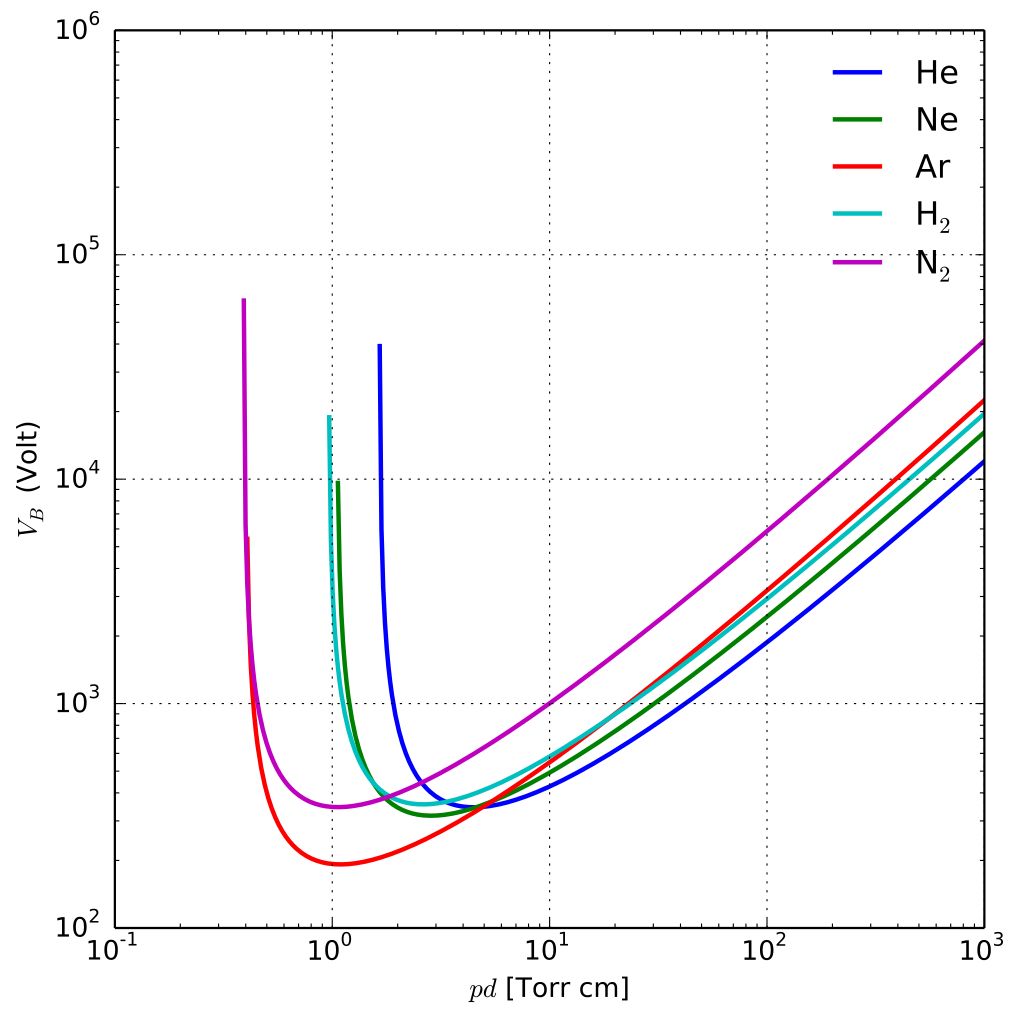
\includegraphics[height=3in]{images/paschencurve.png}
\end{figure}

The breakdown voltage is the voltage required to turn a species into an electrical conductor that allows current to flow through it. I would imagine that a lower breakdown voltage would imply less power is required to create a current through a species.  

\par
When creating an atmospheric plasma it is important to suppress streamers because they cause the plasma to be non-uniform and not helpful for surface plasma treatments because the streamers can damage any surface. A streamer can be thought of as small piece of lightning or what would be observed in one of those tesla coil orbs (a plasma lamp). 

\begin{figure}[H]
\centering
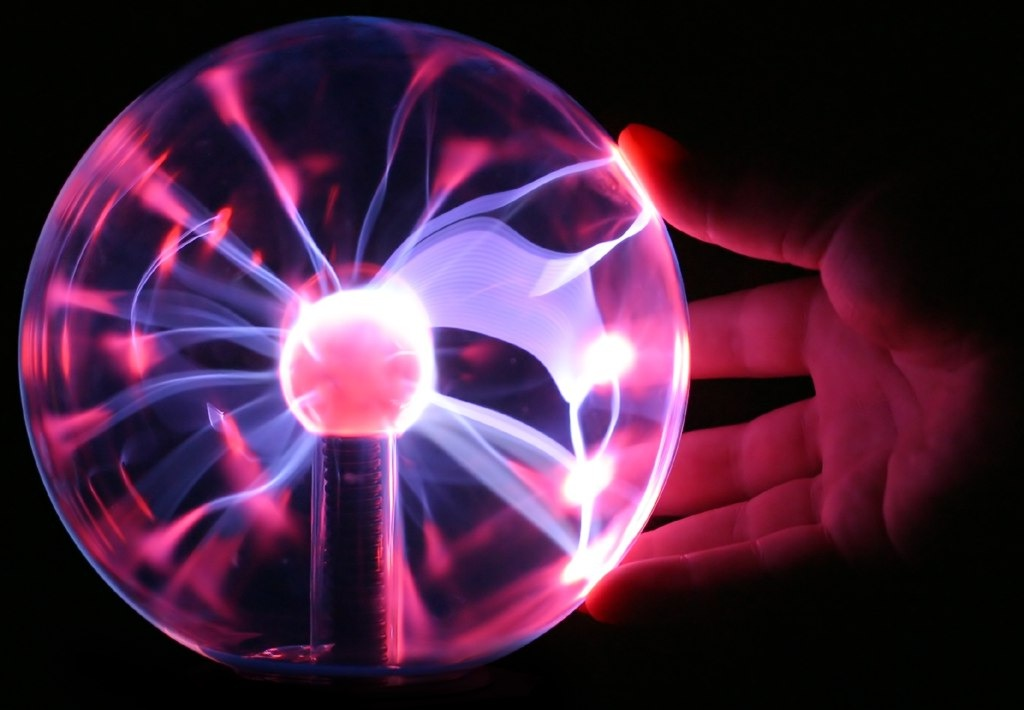
\includegraphics[height=3in]{images/streamerplasma.jpeg}
\end{figure}


\end{document}